\documentclass[12pt,a4paper]{article}
\usepackage{fontspec}
\XeTeXlinebreaklocale "th"
\XeTeXlinebreakskip=0pt plus 1pt
\defaultfontfeatures{Ligatures=TeX}
\setmainfont[
  Path={fonts/TH Sarabun PSK V-1/},
  Extension=.ttf,
  UprightFont={*},
  BoldFont={* Bold},
  ItalicFont={* Italic},
  BoldItalicFont={* BoldItalic}
]{THSarabun}
\setmonofont{Latin Modern Mono}
\usepackage{amsmath,amssymb,mathtools}
\usepackage{unicode-math}
\setmathfont[
  Path={C:/Program Files/MiKTeX/fonts/opentype/public/lm-math/},
  Extension=.otf
]{latinmodern-math}
\usepackage{graphicx,float,caption,xcolor}
\usepackage{geometry,booktabs,tabularx,array,longtable}
\usepackage{tikz}
\usetikzlibrary{arrows.meta,positioning,calc,shapes.geometric}
\usepackage{fancyhdr}
\usepackage[hidelinks]{hyperref}
\geometry{top=0.52in,bottom=0.52in,left=0.58in,right=0.58in}
\setlength{\headheight}{20pt}
\setlength{\parindent}{1.2em}
\setlength{\parskip}{0pt}
\linespread{0.94}
\emergencystretch=2em
\renewcommand{\arraystretch}{1.12}
\captionsetup{font=normalsize,labelfont=bf}
\setlength{\tabcolsep}{4pt}
\pagestyle{fancy}
\fancyhf{}
\lhead{รายงานโครงการระบบไฟฟ้ากำลัง: PF--SSSA--TS--IBR}
\rhead{\thepage}
\renewcommand{\headrulewidth}{0.35pt}
\renewcommand{\figurename}{รูปที่}
\renewcommand{\tablename}{ตารางที่}
\renewcommand{\abstractname}{บทคัดย่อ}
\definecolor{navy}{RGB}{24,54,93}
\definecolor{teal}{RGB}{0,110,112}
\definecolor{redp}{RGB}{165,45,45}
\definecolor{greenp}{RGB}{35,125,67}
\definecolor{goldp}{RGB}{180,139,24}
\definecolor{lightblue}{RGB}{235,244,250}
\definecolor{lightgreen}{RGB}{236,247,239}
\DeclareMathOperator{\sat}{sat}
\newcommand{\pu}{\ensuremath{\,\mathrm{pu}}}
\newcommand{\second}{\ensuremath{\,\mathrm{s}}}
\newcommand{\hz}{\ensuremath{\,\mathrm{Hz}}}
\newcommand{\sci}[2]{\ensuremath{#1\times10^{#2}}}
\newcommand{\reportsection}[1]{\par\addvspace{5pt}{\fontsize{20}{22}\selectfont\bfseries #1\par}\vspace{2pt}}
\newcommand{\source}[1]{\textbf{#1}}
\newcommand{\result}[1]{\textit{#1}}
% Generated by generate_ieee14_gfm_lock_comparison. Do not edit.
% Every number the comparison section prints comes from here, so the prose cannot drift
% from the runs. Arm keys: adaptive, pinned_gfm1, pinned_gfm2, pinned_gfm4, locked_gfl

\newcommand{\ArmAdaptiveLabel}{adaptive}
\newcommand{\ArmAdaptiveHorizon}{250.000}
\newcommand{\ArmAdaptiveConverged}{1}
\newcommand{\ArmAdaptiveReclose}{159.2397}
\newcommand{\ArmAdaptiveGfmMax}{4}
\newcommand{\ArmAdaptiveFailure}{--}
\newcommand{\ArmAdaptiveSamples}{4990}
\newcommand{\ArmAdaptiveRejected}{135}
\newcommand{\DfAdaptiveSGtrip}{0.7587}
\newcommand{\SetAdaptiveSGtrip}{0.0041}
\newcommand{\DfAdaptiveLoadstep}{1.0035}
\newcommand{\SetAdaptiveLoadstep}{0.3753}
\newcommand{\DfAdaptiveFault}{1.1386}
\newcommand{\SetAdaptiveFault}{0.3753}
\newcommand{\DfAdaptiveLinetrip}{0.3764}
\newcommand{\SetAdaptiveLinetrip}{0.3503}
\newcommand{\DfAdaptiveRestorereclose}{1.1612}
\newcommand{\SetAdaptiveRestorereclose}{0.0130}
\newcommand{\ArmPinnedgfmOneLabel}{pinned 1 GFM}
\newcommand{\ArmPinnedgfmOneHorizon}{250.000}
\newcommand{\ArmPinnedgfmOneConverged}{1}
\newcommand{\ArmPinnedgfmOneReclose}{151.4244}
\newcommand{\ArmPinnedgfmOneGfmMax}{1}
\newcommand{\ArmPinnedgfmOneFailure}{--}
\newcommand{\ArmPinnedgfmOneSamples}{3232}
\newcommand{\ArmPinnedgfmOneRejected}{542}
\newcommand{\DfPinnedgfmOneSGtrip}{0.5312}
\newcommand{\SetPinnedgfmOneSGtrip}{0.0113}
\newcommand{\DfPinnedgfmOneLoadstep}{1.4478}
\newcommand{\SetPinnedgfmOneLoadstep}{1.2214}
\newcommand{\DfPinnedgfmOneFault}{1.4979}
\newcommand{\SetPinnedgfmOneFault}{1.2296}
\newcommand{\DfPinnedgfmOneLinetrip}{1.2325}
\newcommand{\SetPinnedgfmOneLinetrip}{1.1426}
\newcommand{\DfPinnedgfmOneRestorereclose}{1.1736}
\newcommand{\SetPinnedgfmOneRestorereclose}{0.0210}
\newcommand{\ArmPinnedgfmTwoLabel}{pinned 2 GFM}
\newcommand{\ArmPinnedgfmTwoHorizon}{250.000}
\newcommand{\ArmPinnedgfmTwoConverged}{1}
\newcommand{\ArmPinnedgfmTwoReclose}{149.9191}
\newcommand{\ArmPinnedgfmTwoGfmMax}{2}
\newcommand{\ArmPinnedgfmTwoFailure}{--}
\newcommand{\ArmPinnedgfmTwoSamples}{3183}
\newcommand{\ArmPinnedgfmTwoRejected}{321}
\newcommand{\DfPinnedgfmTwoSGtrip}{0.3489}
\newcommand{\SetPinnedgfmTwoSGtrip}{0.0001}
\newcommand{\DfPinnedgfmTwoLoadstep}{0.7839}
\newcommand{\SetPinnedgfmTwoLoadstep}{0.7123}
\newcommand{\DfPinnedgfmTwoFault}{0.8255}
\newcommand{\SetPinnedgfmTwoFault}{0.7126}
\newcommand{\DfPinnedgfmTwoLinetrip}{0.7135}
\newcommand{\SetPinnedgfmTwoLinetrip}{0.6422}
\newcommand{\DfPinnedgfmTwoRestorereclose}{0.6634}
\newcommand{\SetPinnedgfmTwoRestorereclose}{0.0209}
\newcommand{\ArmPinnedgfmFourLabel}{pinned 4 GFM}
\newcommand{\ArmPinnedgfmFourHorizon}{25.491}
\newcommand{\ArmPinnedgfmFourConverged}{0}
\newcommand{\ArmPinnedgfmFourReclose}{--}
\newcommand{\ArmPinnedgfmFourGfmMax}{4}
\newcommand{\ArmPinnedgfmFourFailure}{\texttt{adaptiveDtMin}}
\newcommand{\ArmPinnedgfmFourSamples}{819}
\newcommand{\ArmPinnedgfmFourRejected}{449}
\newcommand{\DfPinnedgfmFourSGtrip}{0.9898}
\newcommand{\SetPinnedgfmFourSGtrip}{--}
\newcommand{\DfPinnedgfmFourLoadstep}{--}
\newcommand{\SetPinnedgfmFourLoadstep}{--}
\newcommand{\DfPinnedgfmFourFault}{--}
\newcommand{\SetPinnedgfmFourFault}{--}
\newcommand{\DfPinnedgfmFourLinetrip}{--}
\newcommand{\SetPinnedgfmFourLinetrip}{--}
\newcommand{\DfPinnedgfmFourRestorereclose}{--}
\newcommand{\SetPinnedgfmFourRestorereclose}{--}
\newcommand{\ArmLockedgflLabel}{locked GFL}
\newcommand{\ArmLockedgflHorizon}{20.000}
\newcommand{\ArmLockedgflConverged}{0}
\newcommand{\ArmLockedgflReclose}{--}
\newcommand{\ArmLockedgflGfmMax}{0}
\newcommand{\ArmLockedgflFailure}{\texttt{noVoltageFormingSource}}
\newcommand{\ArmLockedgflSamples}{43}
\newcommand{\ArmLockedgflRejected}{0}
\newcommand{\DfLockedgflSGtrip}{--}
\newcommand{\SetLockedgflSGtrip}{--}
\newcommand{\DfLockedgflLoadstep}{--}
\newcommand{\SetLockedgflLoadstep}{--}
\newcommand{\DfLockedgflFault}{--}
\newcommand{\SetLockedgflFault}{--}
\newcommand{\DfLockedgflLinetrip}{--}
\newcommand{\SetLockedgflLinetrip}{--}
\newcommand{\DfLockedgflRestorereclose}{--}
\newcommand{\SetLockedgflRestorereclose}{--}
\newcommand{\CommonWindowPinnedgfmOneBitIdentical}{1}
\newcommand{\CommonWindowPinnedgfmOneSamples}{42}
\newcommand{\CommonWindowPinnedgfmTwoBitIdentical}{1}
\newcommand{\CommonWindowPinnedgfmTwoSamples}{42}
\newcommand{\CommonWindowPinnedgfmFourBitIdentical}{1}
\newcommand{\CommonWindowPinnedgfmFourSamples}{42}
\newcommand{\CommonWindowLockedgflBitIdentical}{1}
\newcommand{\CommonWindowLockedgflSamples}{42}
\newcommand{\CommonWindowSplit}{20.000}
\newcommand{\CommonWindowAllBitIdentical}{1}
\newcommand{\CandTotal}{15}
\newcommand{\CandReady}{7}
\newcommand{\CandBestSet}{IBR3+IBR6}
\newcommand{\CandBestN}{2}
\newcommand{\CandBestOmega}{-0.56814}
\newcommand{\CandBestSingleOmega}{-0.32801}
\newcommand{\CandFullOmega}{-0.48291}
\newcommand{\CandReadyNOne}{4}
\newcommand{\CandTotalNOne}{4}
\newcommand{\CandReadyNTwo}{2}
\newcommand{\CandTotalNTwo}{6}
\newcommand{\CandReadyNThree}{0}
\newcommand{\CandTotalNThree}{4}
\newcommand{\CandReadyNFour}{1}
\newcommand{\CandTotalNFour}{1}

% Generated by generate_ieee14_report_scalars. Do not edit.
%
% PROVENANCE. Accepted values of output/diagnostics/ieee14_gfm_lock_compare_dcreal/adaptive_250s.mat.
% Produced by run_ieee14_gfm_lock_comparison, whose option set is the
% flagship driver's plus agsi_reference=true (opt-in, post-processing only).
% This cache is NOT bit-identical to the earlier delivered artifact, and no
% such claim is made for it: the DC-link closure changed under
% NUM-2026-08-20-01, so the trajectory legitimately differs. Compare it to
% the earlier cache by outcome, never by bit-identity.
% No value here is rounded, scaled, smoothed or otherwise altered.
%
% Regenerate with:  pf_init_paths; generate_ieee14_report_scalars(result_file="output/diagnostics/ieee14_gfm_lock_compare_dcreal/adaptive_250s.mat")

\newcommand{\NewRunEnd}{250.000}
\newcommand{\NewRunVMin}{0.036855}
\newcommand{\NewRunVMax}{1.523183}
\newcommand{\NewRunFMin}{58.838795}
\newcommand{\NewRunFMax}{61.138560}
\newcommand{\NewRunSubdivision}{0}
\newcommand{\NewRunDomainRejects}{584}
\newcommand{\NewRunResidual}{$9.9596\times10^{-9}$}
\newcommand{\NewRunReclose}{159.240}
\newcommand{\NewRunRecloseStatus}{SUCCESS}
\newcommand{\NewRunSyncDV}{0.008785}
\newcommand{\NewRunSyncDF}{$6.4601\times10^{-13}$}
\newcommand{\NewRunSyncDTheta}{5.015017}
\newcommand{\NewRunFirstRelease}{25.310}
\newcommand{\NewRunReleaseOne}{25.310}
\newcommand{\NewRunReleaseTwo}{146.247}
\newcommand{\NewRunReleaseThree}{152.390}
\newcommand{\NewRunReleaseFour}{--}
\newcommand{\NewRunAugmentOne}{22.052}
\newcommand{\NewRunAugmentTwo}{51.333}
\newcommand{\NewRunAugmentThree}{53.372}
\newcommand{\NewRunAugmentFour}{148.267}
\newcommand{\NewRunNRelease}{3}
\newcommand{\NewRunNAugment}{4}
\newcommand{\NewRunGfmMax}{4}
\newcommand{\NewRunSamples}{4990}
\newcommand{\NewRunRejectedSteps}{135}
\newcommand{\NewRunTerminalF}{60.000000}
\newcommand{\NewRunTerminalVMin}{0.9667}
\newcommand{\NewRunTerminalVMax}{1.0575}
\newcommand{\NewRunStepper}{adaptive}
\newcommand{\NewRunReselection}{NO\_FEASIBLE\_SG\_ON\_ONE\_STEP}

\graphicspath{{figures/}{figures/final_report_th/}}

\begin{document}`r`n\makeatletter`r`n\renewcommand\normalsize{\fontsize{18}{19.2}\selectfont}`r`n\makeatother`r`n\normalsize

\begin{titlepage}
\thispagestyle{empty}
\begin{center}
\vspace*{0.55in}

\includegraphics[width=1.08in]{figures/images.png}\\[0.35in]
{\color{navy}\fontsize{25}{31}\selectfont\bfseries
รายงานโครงการระบบไฟฟ้ากำลัง\par}
\vspace{0.10in}
{\color{teal}\fontsize{20}{25}\selectfont\bfseries
การไหลของกำลัง การวิเคราะห์เสถียรภาพ และการสลับโหมด GFL/GFM อัตโนมัติ\par}
\vspace{0.12in}
{\color{navy}\fontsize{16}{20}\selectfont
กรณีศึกษา IEEE 14-bus: PF, SSSA, TS และ IBR แบบผสม\par}
\vspace{0.50in}
\rule{4.7in}{0.8pt}\\[0.30in]
{\fontsize{15}{19}\selectfont
Mr. Phichitchai Jueajan (66010569)\\
Mr. Pakkapol Phdungdan (66010612)\par}
\vspace{0.22in}
{\fontsize{14}{18}\selectfont
อาจารย์ที่ปรึกษา: Dr.\ Tossaporn Surinkaew\\
อาจารย์ที่ปรึกษาร่วม: Prof.\ Dr.\ Issarachai Ngamroo\par}
\vfill
{\fontsize{13}{17}\selectfont
ภาควิชาวิศวกรรมไฟฟ้า คณะวิศวกรรมศาสตร์\\
สถาบันเทคโนโลยีพระจอมเกล้าเจ้าคุณทหารลาดกระบัง\par}
\vspace{0.32in}
{\fontsize{12}{15}\selectfont สิงหาคม พ.ศ. 2569\par}
\end{center}
\end{titlepage}

\reportsection{บทคัดย่อ วัตถุประสงค์ และขอบเขตข้ออ้าง}
\begin{abstract}
โครงการนี้พัฒนาสายงานคำนวณระบบไฟฟ้ากำลังภายในโครงการเดียว ตั้งแต่การแก้
สมการการไหลของกำลัง (PF) ไปยังจุดสมดุลของระบบสมการเชิงอนุพันธ์--พีชคณิต
(DAE) การวิเคราะห์เสถียรภาพสัญญาณขนาดเล็ก (SSSA) และการจำลองโดเมนเวลา (TS)
ด้วยตัวแก้สมการ MATLAB แบบฐานล้วนของโครงการ จากนั้นนำ DAE เดียวกันไปทดสอบ
เครือข่าย IEEE-14 ที่มี synchronous generator (SG) หนึ่งเครื่องและ
inverter-based resource (IBR) สี่ตัว ซึ่งสลับระหว่าง grid-following (GFL)
และ grid-forming (GFM) โดย supervisor ที่มี hysteresis, dwell และ guard
สำหรับเจ้าของมุมอ้างอิง

ผลหลักมาจาก cache หกแขนชุดเดียวที่ commit \texttt{c56ff9f} และสร้างรูปใหม่
ด้วยตัวอ่าน cache ที่ตรวจ hash ก่อนและหลังอ่าน ค่าในตารางและรูปจึงเป็นค่าที่
ตัวแก้ยอมรับจริง ไม่มีการทำให้เรียบ การเติมสัญญาณ หรือการตัดข้อมูล การรัน
adaptive ไปถึง \ArmAdaptiveHorizon\ วินาที ปิด SG ได้และ reclose ที่
\ArmAdaptiveReclose\ วินาที ขณะที่แขนที่ตรึง GFM สี่ตัวตั้งแต่ต้นหยุดที่
\ArmPinnedgfmFourHorizon\ วินาที ตัวเลขเหล่านี้เป็น \result{PROJECT\_RESULT}
ของแบบจำลอง ไม่ใช่การรับรองการใช้งานภาคสนาม
\end{abstract}

\paragraph{วัตถุประสงค์}
(1) ทำให้สมการ PF--SSSA--TS ใช้ residual และลำดับตัวแปรเดียวกัน
(2) แสดงหลักฐาน independent ของ equilibrium, Schur complement และ
finite-difference (FD) Jacobian
(3) ตรวจสัญญา IBR GFL/GFM และการถ่ายโอน state โดยไม่ให้กระแสกระโดด
และ (4) รายงานผล chronology 250 วินาทีพร้อมการเปรียบเทียบนโยบายหกแขนอย่าง
ตรวจสอบย้อนกลับได้

\paragraph{ขอบเขตข้ออ้าง}
ข้อมูล network และเหตุการณ์ที่ระบุว่า \source{SOURCE\_DEFINED} หรือ
\source{CASE\_DEFINED} ถูกใช้ตามต้นทาง ผลของตัวแก้เป็น
\result{PROJECT\_RESULT} และสมการ/การปิดที่เจ้าของโครงการกำหนดถูกระบุเป็น
\source{PROJECT\_DERIVED} หรือ \source{NUMERICAL\_METHOD} รายงานนี้ไม่อ้าง
grid-code compliance, protection coordination, EMT accuracy หรือ readiness
สำหรับการใช้งานจริง

\paragraph{การทำซ้ำ}
รายงานภาษาไทยอ่าน macro ที่สร้างจาก cache โดยตรงและอ่าน PNG ที่ตัวสร้าง
รายงานสร้างขึ้นใหม่ ทุกค่าในหน้าต่อไปจึงผูกกับ provenance เดียวกัน ไม่ใช่
การคัดตัวเลขจากรายงานฉบับก่อน

\par\vspace{5pt}

\reportsection{จุดเริ่มต้นของโครงการและ milestone สำคัญ}
จุดเริ่มต้นคือปัญหาที่การสูญเสีย SG ทำให้โครงข่ายไม่มีแหล่งกำหนดแรงดัน
อ้างอิง GFL ต้องอาศัย PLL ส่วน GFM สร้างมุมและแรงดันของตนเอง โครงการจึง
วางสายงานแบบลำดับชั้น: PF สร้าง operating point, equilibrium ปิด KCL และ
สมการ device, SSSA ตรวจการรบกวนเล็ก, TS ตรวจเหตุการณ์ขนาดใหญ่ และ supervisor
ตัดสินใจ mode จาก state ที่ยอมรับแล้ว

\begin{table}[H]
\centering
\caption{ลำดับพัฒนาการที่ใช้เป็นหลักฐานในรายงานนี้}
\begin{tabularx}{\textwidth}{@{}c p{0.25\textwidth} X@{}}
\toprule
ลำดับ & milestone & หลักฐานและความหมาย \\
\midrule
1 & สัญญา base และ bus type & power-case 1.0, bus 12 คอลัมน์, REF/PV/PQ เป็น 1/2/3 \\
2 & Ybus และ PF Newton & residual $[P,Q]$ มี mapping และ limit ที่ตรวจย้อนกลับได้ \\
3 & shared DAE & equilibrium, SSSA และ TS เรียก residual เดียวกัน \\
4 & SSSA Schur & กำจัดตัวแปร algebraic ด้วย backslash และตรวจ conditioning \\
5 & FD/eigenpair gates & ตรวจ plateau, conjugate pair, gauge และ participation \\
6 & implicit trapezoidal TS & corrector แก้ differential และ KCL พร้อมกัน \\
7 & event landing & แต่ละ event ลงตรง grid และเปลี่ยน topology แบบ right-limit \\
8 & GFL-RMS10 SMIB & ปิด nonlinear PLL, current plant และ power identity แยกกรณี \\
9 & GFM no-PLL SMIB & ปิด VSG angle และ voltage law โดยไม่มี PLL แฝง \\
10 & dual-mode 17-state & plant ร่วมและ controller block ที่ active ได้ทีละ branch \\
11 & IEEE-14 integration & SG bus 1 กับ IBR bus 2, 3, 6, 8 ใน composite DAE \\
12 & six-arm snapshot & เปรียบเทียบ adaptive, pinned และ no-adaptation จาก cache เดียว \\
\bottomrule
\end{tabularx}
\end{table}

\paragraph{หลักวินัยข้อมูล}
external PSAT, PGAz และเอกสารอ้างอิงใช้เป็น oracle หรือ comparison เท่านั้น
ไม่ถูกเรียกจาก production path และผลจากภายนอกไม่ถูกป้อนกลับไปเลือก state,
parameter, correction หรือ gate การเปลี่ยนแปลงของรายงานนี้จำกัดอยู่ที่
report-only generator และเอกสาร จึงไม่เปลี่ยน numerical contract

\paragraph{จุดที่ไม่ถูกนำมาอ้าง}
ตัวนับ trial ที่ถูกปฏิเสธใน search path มี defect record เปิดอยู่ จึงไม่นำ
ตัวเลขดังกล่าวมาสนับสนุนข้ออ้างใดในรายงานนี้ การเปรียบเทียบใช้ accepted
samples, horizon, residual และสถานะ convergence ซึ่งเป็นค่าที่ตรวจซ้ำได้

\par\vspace{5pt}

% ============================================================================
% 4. Architecture and numerical integrity
\reportsection{สถาปัตยกรรม PF ถึงการสลับโหมด และหลัก numerical integrity}
\begin{figure}[H]
\centering
\begin{tikzpicture}[
  node distance=0.18in and 0.12in,
  box/.style={draw=navy,fill=lightblue,rounded corners=2pt,
    minimum width=1.18in,minimum height=0.65in,align=center},
  gate/.style={draw=teal,fill=lightgreen,rounded corners=2pt,
    minimum width=1.30in,minimum height=0.65in,align=center},
  arr/.style={-{Latex[length=2.5mm]},very thick,draw=navy}
]
\node[box] (data) {case data\\และฐานหน่วย};
\node[box,right=of data] (pf) {PF Newton\\$P,Q$ residual};
\node[box,right=of pf] (eq) {equilibrium\\$f=0,\;g=0$};
\node[box,right=of eq] (ssa) {SSSA\\Schur + eigenpairs};
\node[box,right=of ssa] (ts) {TS\\trapezoidal + KCL};
\node[gate,below=0.45in of ts] (switch) {supervisor\\GFL/GFM + guard};
\node[gate,left=of switch] (events) {events\\right-limit};
\node[gate,left=of events] (qa) {accepted state\\provenance};
\draw[arr] (data)--(pf)--(eq)--(ssa)--(ts);
\draw[arr] (ts)--(switch);
\draw[arr] (switch)--(events);
\draw[arr] (events)--(qa);
\draw[arr] (qa) |- (eq.south);
\node[below=0.17in of pf,align=center,text=navy] {one in-house\\residual owner};
\node[below=0.17in of eq,align=center,text=navy] {same state order\\for SSSA/TS};
\end{tikzpicture}
\caption{สถาปัตยกรรมที่ใช้จริง: PF สร้างจุดตั้งต้น, equilibrium ปิด DAE,
SSSA และ TS ใช้สมการเดียวกัน และ supervisor เปลี่ยน mode เฉพาะที่ accepted
right-limit}
\end{figure}

\paragraph{ตัวแปรและสัญญา}
ให้ $x$ เป็น differential state, $y$ เป็น rectangular bus-voltage state
เรียงเป็น $[\operatorname{Re}V_1,\operatorname{Im}V_1,\ldots]$ และ $u$ เป็น
input ของ device ระบบแก้
\begin{equation}
\dot{x}=f(x,y,u),\qquad 0=g(x,y,u).
\end{equation}
กระแสของ device เป็นบวกเมื่อฉีดเข้าสู่ network และ
$S=V I^{*}=P+\mathrm{j}Q$ บน system base สัญญานี้ไม่เปลี่ยนเมื่อเปลี่ยน
เครื่องมือ comparison

\paragraph{การปิดแบบ fail-closed}
ทุก stage ตรวจ finite state, residual, rank/conditioning และ mapping ก่อน
commit หากเงื่อนไขไม่ผ่านจะหยุดและเก็บ failure status ตัวอย่างสำคัญคือ
การไม่มี voltage-forming source หลัง SG trip และการที่ Newton step ลง domain
ไม่ได้รับการแก้ด้วยการผ่อน gate

\paragraph{การจำแนกค่า}
\source{SOURCE\_DEFINED} ใช้เมื่อแหล่งอ้างอิงระบุสมการหรือค่าโดยตรง
\source{CASE\_DEFINED} ใช้กับ case และ event
\source{PROJECT\_DERIVED} ใช้กับ closure ที่ต้องพิสูจน์ด้วยสมการ
\source{NUMERICAL\_METHOD} ใช้กับวิธีแก้และ tolerance
และ \source{ASSUMED\_DIAGNOSTIC} ใช้กับดัชนีที่แสดงเพื่อวิเคราะห์เท่านั้น

\par\vspace{5pt}


% ============================================================================
% 5. PF method
\reportsection{วิธีแก้ Power Flow: สมการ ตัวแปร และเกณฑ์หยุด}
สำหรับ bus $i$ ให้ $V_i=|V_i|e^{\mathrm{j}\theta_i}$ และ
$Y=G+\mathrm{j}B$ สมการกำลังที่ production ใช้คือ
\begin{align}
P_i&=\sum_k |V_i||V_k|
 (G_{ik}\cos\theta_{ik}+B_{ik}\sin\theta_{ik}),\\
Q_i&=\sum_k |V_i||V_k|
 (G_{ik}\sin\theta_{ik}-B_{ik}\cos\theta_{ik}),
\end{align}
โดย $\theta_{ik}=\theta_i-\theta_k$ และ
$P_i^{\mathrm{spec}}=P_{G,i}-P_{L,i}$,
$Q_i^{\mathrm{spec}}=Q_{G,i}-Q_{L,i}$

\begin{table}[H]
\centering
\caption{บทบาทของ bus และ unknown ใน Newton--Raphson}
\begin{tabularx}{\textwidth}{@{}l l X@{}}
\toprule
ประเภท & ค่าที่กำหนด & ค่าที่แก้หรือรายงาน \\
\midrule
REF & $|V|,\theta$ & $P,Q$ เป็นผลลัพธ์ของ balance \\
PV & $P,|V|$ & $\theta$ แก้; $Q$ รายงานและตรวจ limit \\
PQ & $P,Q$ & $\theta,|V|$ แก้ \\
\bottomrule
\end{tabularx}
\end{table}

Mismatch vector เรียงเฉพาะค่าที่ไม่ถูกกำหนด:
\begin{equation}
r_{\mathrm{PF}}=
\begin{bmatrix}P^{\mathrm{spec}}-P^{\mathrm{calc}}\\
Q^{\mathrm{spec}}-Q^{\mathrm{calc}}\end{bmatrix},
\qquad
J=
\begin{bmatrix}H&N\\M&L\end{bmatrix}
=\frac{\partial r_{\mathrm{PF}}}{\partial[\theta\;\;|V|]}.
\end{equation}
แต่ละรอบแก้ $J\Delta z=r_{\mathrm{PF}}$ ด้วย backslash แล้วอัปเดต
$z\leftarrow z+\Delta z$ จน $\|r_{\mathrm{PF}}\|_\infty$ ต่ำกว่า tolerance
ที่ประกาศไว้

\paragraph{Limits และการหยุด}
เมื่อ reactive generation ของ PV ออกนอก $[Q_{\min},Q_{\max}]$ ค่า $Q$ จะถูก
ตรึงที่ limit และ bus เปลี่ยนเป็น PQ ก่อนแก้ต่อ REF ไม่ถูกใช้เป็น unknown
แรงดันและมุมที่ได้จึงยังเป็น output ของสมการ ไม่ใช่ค่าที่ป้อนกลับจาก oracle
การประกอบ $Y$ รวม series admittance, shunt, line charging และ transformer tap
ตาม case data และตรวจ power balance
$P_{\mathrm{gen}}=P_{\mathrm{load}}+P_{\mathrm{loss}}$

\paragraph{หน่วย}
ค่ากำลังใช้ pu บนฐาน 100 MVA ของ case; แรงดันและกระแสใช้ pu; มุมแสดงเป็น
องศาแต่สมการใช้เรเดียน ความแตกต่างของ frame หรือ sign จึงถูกตรวจที่ residual
ก่อนจะนำไป SSSA หรือ TS

\paragraph{หลักฐาน independent}
PF production เป็น Newton ภายในโครงการ ส่วน PSAT/MATPOWER/PGAz ถูกใช้เพื่อ
อ่านหรือเปรียบเทียบข้อมูลเท่านั้น การตรงกันของค่าภายนอกจึงเป็น diagnostic
ไม่ใช่ source ของ correction

\par\vspace{5pt}


% ============================================================================
% 6. PF evidence
\reportsection{หลักฐาน PF: IEEE-14, RTS-24 และ comparison ที่รายงานตามจริง}
\begin{table}[H]
\centering
\caption{ผล PF จาก artifact ที่สร้างสดและ mapping เดียวกับ production}
\begin{tabularx}{\textwidth}{@{}l r r r r X@{}}
\toprule
กรณี & สถานะ & รอบ Newton & $\|r_{\mathrm{PF}}\|_\infty$ & $P_G$ (pu) & balance \\
\midrule
IEEE-14 & converged & 5 & $\sci{6.33521}{-15}$ & 2.72393 &
$P_L=2.59000,\;P_{\mathrm{loss}}=0.133933$ \\
RTS-24 & converged & 5 & $\sci{2.30926}{-12}$ & 29.0125 &
$P_L=28.5000,\;P_{\mathrm{loss}}=0.512464$ \\
\bottomrule
\end{tabularx}
\end{table}

\paragraph{IEEE-14}
เครือข่ายหลักใช้ bus ID จาก case14 และรักษา semantic ของ REF/PV/PQ ก่อน
ส่งผลให้ equilibrium ของ SG bus 1 และ IBR bus 2, 3, 6, 8 ถูกสร้างใน coordinate
ชุดเดียวกับ composite DAE ค่า residual ที่ต่ำกว่า
$\sci{10}{-14}\pu$ เป็นหลักฐาน numerical convergence ของ operating point
ไม่ใช่หลักฐานว่า parameter ของ SG เป็นค่าจากโรงงาน

\paragraph{RTS-24}
RTS-24 ใช้เป็นกรณีข้ามขนาดเพื่อจับ error ใน bus/branch mapping, power balance
และการแยก state ออกจาก algebraic variable ไม่ได้ใช้ผล RTS-24 ไป tune
IEEE-14 การเทียบข้ามกรณีจึงเป็นการตรวจ implementation contract

\paragraph{การเทียบ PSAT และ PGAz}
ใน fixed-grid IEEE-14 fault test ค่า PSAT--Ours สูงสุดคือ
$\Delta\mathrm{COI}=\sci{9.5711}{-3}$ องศา,
$\Delta\omega=\sci{3.8160}{-6}\pu$,
$\Delta P_e=0.042171$ MW และ
$\Delta V=\sci{3.1793}{-5}\pu$ ซึ่งอยู่ใน primary tolerance ที่ประกาศ
PGAz ทำงานจบแต่ต่างมากกว่า: $\Delta\mathrm{COI}=0.616348$ องศาและ
$\Delta P_e=2.467655$ MW จึงรายงานเป็น secondary diagnostic ไม่ได้ซ่อน
ด้วยการผ่อน tolerance

\paragraph{PGAz FAIL ตามจริง}
artifact ระบุว่า PGAz execution ผ่าน แต่ corrector ไม่ส่ง residual และ gate
ของ trajectory comparison ไม่ผ่าน การเขียนว่า "ผ่านทั้งหมด" จะเกิน
หลักฐาน จึงใช้คำว่า comparison diagnostic เท่านั้น

\par\vspace{5pt}


% ============================================================================
% 7. SSSA method
\reportsection{วิธี SSSA: DAE, Schur complement, eigenpairs และ participation}
ที่ equilibrium $(x_0,y_0)$ มี $f(x_0,y_0)=0$ และ $g(x_0,y_0)=0$
การรบกวนอันดับหนึ่งให้
\begin{equation}
\begin{bmatrix}\Delta\dot{x}\\0\end{bmatrix}=
\begin{bmatrix}J_{xx}&J_{xy}\\J_{yx}&J_{yy}\end{bmatrix}
\begin{bmatrix}\Delta x\\\Delta y\end{bmatrix}.
\end{equation}
เมื่อ $J_{yy}$ อยู่ใน free algebraic set, production กำจัด $\Delta y$ ด้วย
\begin{equation}
A=J_{xx}-J_{xy}
\left(J_{yy}\right)^{-1}J_{yx}
\quad\Longrightarrow\quad
A=J_{xx}-J_{xy}\left(J_{yy}\backslash J_{yx}\right)
\end{equation}
โดยรูปที่สองคือรูปที่ใช้จริงและไม่มีการสร้าง explicit inverse

\paragraph{FD Jacobian}
แต่ละ block ของ $J$ ได้จาก central FD รอบ equilibrium ด้วย step ที่ตรึงไว้
การเลือก step อาศัย plateau ของ eigenvalues ที่วัดได้ ไม่ได้อาศัยการปรับให้
ตรงกับหนังสือหรือโปรแกรมอ้างอิง Eigenpair residual, conjugate pairing,
conditioning และ reference-angle structure เป็น gates แยกกัน

\paragraph{Gauge และ reduction}
ระบบ autonomous มี rotational symmetry จึงมี zero mode ของการเลื่อนมุมร่วม
full matrix เก็บ mode นี้ ส่วน COI reduction ใช้เมื่อโจทย์ต้องการ modes
ที่ตัด common motion การอ่าน damping ใช้
\begin{equation}
\lambda=\sigma+\mathrm{j}\varpi,\qquad
f_\lambda=\frac{|\varpi|}{2\pi},\qquad
\zeta=-\frac{\sigma}{|\lambda|}.
\end{equation}
ถ้า $\operatorname{Re}\lambda<0$ mode ลดลง; ถ้าไม่ finite หรืออยู่อีกฝั่ง
ต้อง fail-closed ไม่ตีความเป็น stable

\paragraph{Participation}
left/right eigenvectors ใช้เพื่อจัดอันดับ state ที่เด่นเท่านั้น หาก conditioning
ไม่พอผล participation จะถูกทำเครื่องหมาย unavailable การจัดอันดับนี้ไม่
เปลี่ยน eigenvalue, candidate set หรือ solver state

\paragraph{หลักฐานจาก shared path}
SSSA เรียก DAE เดียวกับ TS บนลำดับ $(x,y)$ เดียวกัน ดังนั้น residual ที่ถูก
ตรวจใน SSSA ไม่ใช่ residual ที่สร้างขึ้นเพื่อรายงาน หลังจาก SSSA ผ่านจึงนำ
equilibrium เดิมไปเริ่ม TS โดยไม่ copy ค่า eigenvalue หรือ reference table

\par\vspace{5pt}


% ============================================================================
% 8. SSSA evidence
\reportsection{หลักฐาน SSSA: residual, FD plateau, gates และ Padiyar discrepancy}
\begin{table}[H]
\centering
\caption{ค่าหลักจาก SSSA validation artifact}
\begin{tabularx}{\textwidth}{@{}l r r r r X@{}}
\toprule
แบบจำลอง & $\max|f_0|$ & $\max|g_0|$ & จำนวน state & จำนวน eigenvalue & FD plateau \\
\midrule
Padiyar manual & $\sci{1.249}{-15}$ & $\sci{5.684}{-14}$ & 16 & 16 &
$\sci{1.686}{-7}$ \\
Padiyar AVR & $\sci{9.215}{-13}$ & $\sci{5.684}{-14}$ & 20 & 20 &
$\sci{5.799}{-9}$ \\
EMF6 & $\sci{1.665}{-15}$ & $\sci{2.132}{-14}$ & 24 & 24 &
$\sci{1.078}{-7}$ \\
\bottomrule
\end{tabularx}
\end{table}

ค่าทั้งหมดต่ำกว่า $\sci{10}{-10}$ ที่ equilibrium และ eigenvalues finite
ทุกตัว Schur reconstruction ของ Padiyar AVR ให้ความต่างเชิงตัวเลขเป็นศูนย์
และ $J_{yy}$ มี rcond ประมาณ $\sci{9.74}{-3}$ สำหรับ Padiyar กับ
$\sci{1.11}{-2}$ สำหรับ EMF6 จึงไม่ใช่การแก้ระบบที่เกือบ singular

\paragraph{FD plateau}
การเปรียบเทียบ $h=10^{-5}$ กับ $h=10^{-6}$ ให้ความต่าง physical modes
ตามตาราง โดยค่าทั้งหมดต่ำกว่า $\sci{10}{-3}$ ที่ประกาศไว้ default step
ของ production อยู่บน plateau นี้

\paragraph{Gate matrix}
รายการ gate ของ SSSA validation artifact ผ่านทั้งหมด ครอบคลุม shared DAE,
state order/count, FD convergence, default-on-plateau, Schur solve,
ไม่มี explicit inverse, gauge, conjugate pair, modal metrics,
reference independence, provenance และ no external solver การทดสอบที่
บันทึกไว้คือ targeted 62 ผ่าน, 0 ไม่ผ่าน, 0 incomplete; ตัวเลขนี้เป็น
evidence ของ code path เดิม ไม่ใช่การรันซ้ำเพื่อให้รายงานผ่าน

\paragraph{Padiyar discrepancy}
การจับคู่ Table 9.5 ของ Padiyar เป็น \source{ASSUMED\_DIAGNOSTIC} แบบ
greedy one-to-one เท่านั้น มี 18 physical roots และความต่างสูงสุดประมาณ
$\sci{4.3}{-2}$ การตรวจ FD plateau อยู่ระดับ $\sci{10}{-7}$ จึงอธิบาย
ความต่าง $\sci{4.3}{-2}$ ด้วย FD noise ไม่ได้ สาเหตุที่แท้จริงยังไม่ปิด
อาจเกี่ยวกับ model, data, convention หรือ precision ของสิ่งพิมพ์ รายงาน
ความต่างนี้ตรง ๆ และไม่ใช้เป็น acceptance gate

\par\vspace{5pt}


% ============================================================================
% 9. TS method
\reportsection{วิธี TS: implicit trapezoidal, corrector, event landing และ COI}
สำหรับช่วงที่ topology คงที่ production ใช้ implicit trapezoidal:
\begin{equation}
R_x=x_{n+1}-x_n-\frac{h}{2}
\left[f(t_n,x_n,y_n)+f(t_{n+1},x_{n+1},y_{n+1})\right]=0,
\qquad
R_g=g(t_{n+1},x_{n+1},y_{n+1})=0.
\end{equation}
Newton corrector แก้ $[R_x;R_g]$ พร้อมกันจน update และ residual ผ่าน
ตัวแก้ EMF6 ใช้ corrector iteration คงที่สามรอบตาม contract ส่วน adaptive
stepper ใช้ step-doubling เพื่อประมาณ local error และยอมรับ fine solution
เมื่อ weighted error และ KCL residual ผ่าน

\begin{figure}[H]
\centering
\begin{tikzpicture}[
  box/.style={draw=navy,fill=lightblue,rounded corners=2pt,
    minimum width=1.68in,minimum height=0.70in,align=center},
  arr/.style={-{Latex[length=2.5mm]},very thick,draw=navy}
]
\node[box] (left) {$t_n$\\left topology\\accepted $(x_n,y_n)$};
\node[box,right=0.65in of left] (step) {predict + Newton\\solve $R_x,R_g$};
\node[box,right=0.65in of step] (right) {$t_{n+1}$\\accepted right limit};
\node[box,below=0.45in of step] (event) {ถ้า $t_{n+1}=t_e$\\apply event transaction};
\draw[arr] (left)--(step)--(right);
\draw[arr] (step)--(event);
\draw[arr] (event)--(right);
\end{tikzpicture}
\caption{แต่ละ step แก้ DAE บน topology เดียว; event ที่ลง grid ใช้
left topology สำหรับ arrival และ re-solve right topology แบบ atomic}
\end{figure}

\paragraph{Exact event landing}
ถ้า event อยู่ก่อนปลาย step จะลด $h$ ให้ลงตรง event เสมอ ห้าม step เดียว
คร่อมสอง topology เมื่อเปลี่ยน mode จะ carry plant state, initialize
controller block ของปลายทาง และตรวจ terminal-current continuity
\begin{equation}
|I^{+}-I^{-}|\le \sci{10}{-10}\pu.
\end{equation}
ถ้า right-limit Newton หรือ continuity gate ไม่ผ่าน transaction ถูก rollback
ทั้งชุด

\paragraph{COI metrics}
สำหรับเครื่องที่มี inertia $H_i$ ใช้
$\delta_{\mathrm{COI}}=\sum_iH_i\delta_i/\sum_iH_i$ และ
$f_{\mathrm{COI}}$ เป็น frequency metric ของระบบ การลบ common motion นี้
ใช้กับ comparison เท่านั้น ไม่เปลี่ยน state ที่ตัวแก้ integrate

\paragraph{Adaptive policy}
ตัวควบคุมเวลาเลือก $h_{\mathrm{new}}$ จาก error ที่ normalize ด้วย
$\mathrm{atol}+\mathrm{rtol}\max|x|$ และจำกัดอัตราขยาย/หดตามค่าที่ประกาศ
เมื่อ reject จะไม่เขียนทับ accepted state ไม่มี extrapolation ของ arm ที่หยุด
ก่อน horizon

\par\vspace{5pt}


% ============================================================================
% 10. TS evidence
\reportsection{หลักฐาน TS: common grid, IEEE-14 และ RTS-24}
\begin{table}[H]
\centering
\caption{ผล comparison บน common grid ที่ไม่ extrapolate}
\begin{tabularx}{\textwidth}{@{}l l r r r r@{}}
\toprule
คู่เทียบ & metric & $\max|\Delta\mathrm{COI}|$ (deg) &
$\max|\Delta\omega|$ (pu) & $\max|\Delta P_e|$ (MW) &
$\max|\Delta V|$ (pu) \\
\midrule
PSAT--Ours & IEEE-14 & 0.009571 & $\sci{3.816033}{-6}$ & 0.042171 &
$\sci{3.179264}{-5}$ \\
PGAz--Ours & IEEE-14 & 0.616348 & $\sci{2.916429}{-4}$ & 2.467655 &
$\sci{2.264528}{-3}$ \\
PSAT--Ours & RTS-24 & 0.0067685 & $\sci{4.6205}{-6}$ & 0.082705 &
$\sci{5.3538}{-6}$ \\
\bottomrule
\end{tabularx}
\end{table}

\paragraph{วิธีอ่านตาราง}
กริดเปรียบเทียบใช้ event และ sample time ที่มีอยู่จริงของแต่ละ solver
ห้าม extrapolate ออกนอกช่วงที่ solver ให้มา ค่า PSAT--Ours ของ IEEE-14
อยู่ใต้ tolerance ที่ประกาศ จึงเป็น primary comparison ส่วน PGAz มี
trajectory difference ใหญ่กว่าและ corrector residual ไม่พร้อมให้ยืนยัน
ดังนั้นเป็น diagnostic เท่านั้น

\paragraph{RTS-24 เป็น held-out check}
RTS-24 ตรวจว่าการประกอบ network, constant-impedance conversion ที่ runtime,
COI mapping และ event landing ไม่ผูกกับจำนวน bus ของ IEEE-14 ผลที่ต่างจาก
PSAT ถูกพิมพ์เป็น metric ไม่ถูกใช้เพื่อเปลี่ยน solver

\paragraph{สิ่งที่ TS พิสูจน์และไม่พิสูจน์}
TS พิสูจน์ว่า accepted DAE state มี residual และ event order ตามสัญญา
แต่ไม่ได้พิสูจน์ hardware control, protection, unbalanced fault หรือ
accuracy ของ switching waveform ระดับ EMT นอกจากนี้ fixed-step และ adaptive
เป็น numerical routes ที่ต้องอ่านแยกกัน ไม่สรุปว่าการรันสั้นรับรอง horizon ยาว

\begin{center}
\fcolorbox{teal}{lightgreen}{\begin{minipage}{0.90\textwidth}
\textbf{ข้อสรุปหน้านี้:} common-grid comparison ผ่านในส่วน PSAT primary
ตามตัวเลขที่วัดได้ ส่วน PGAz ถูกเก็บไว้เพื่อบอกขอบเขตของความสอดคล้อง ไม่ใช่
ถูกลบหรือปรับ tolerance ให้ดูดี
\end{minipage}}
\end{center}

\par\vspace{5pt}


% ============================================================================
% 11. IBR development
\reportsection{พัฒนาการ IBR: GFL+PLL, GFM no-PLL, 17-state superset}
IBR แต่ละตัวมี plant ร่วมและ controller สอง branch แต่ integrate branch เดียว
ในเวลาใดเวลาหนึ่ง GFL ใช้ current control และ SRF-PLL ส่วน GFM ใช้ VSG
swing และ voltage-forming loop การเลือก mode ไม่ได้หมายความว่าสอง controller
ทำงานพร้อมกัน

\begin{align}
x_{\mathrm{GFL}}&=[\,\delta_{\mathrm{PLL}},\xi_{\mathrm{PLL}},
\xi_P,\xi_Q,\xi_{Id},\xi_{Iq}\,],\\
x_{\mathrm{GFM}}&=[\,\delta_{\mathrm{VSG}},\omega_{\mathrm{VSG}},E,
\xi_{Vd},\xi_{Vq},\xi_{Id},\xi_{Iq}\,].
\end{align}
plant ร่วมคือ $(i_d,i_q,V_{dc})$ และ source-current state $I_{dc}$ ถูก append
เป็นพิกัดที่ 17 สร้าง fixed superset 17 state
\begin{equation}
x_{\mathrm{IBR}}\in\mathbb{R}^{17},\qquad
\mathcal{A}_{\mathrm{GFL}}=\{1{:}9,17\},\quad
\mathcal{A}_{\mathrm{GFM}}=\{1{:}3,10{:}16,17\}.
\end{equation}
ดังนั้น active count เป็น 10 หรือ 11 ไม่ใช่ 17 พร้อมกัน

\paragraph{GFL}
PLL ขับ $v_q$ เป็นศูนย์และใช้ $\omega_{\mathrm{PLL}}$ เป็น frame frequency
outer $P/Q$ loops สร้าง current reference ส่วน inner loops แก้ filter current
ที่ equilibrium $P$ และ $Q$ ตรง setpoint จาก source

\paragraph{GFM no-PLL}
VSG ให้
\begin{equation}
M\dot{\omega}_{\mathrm{VSG}}=\kappa P_{\mathrm{ref}}-P_{\mathrm{inv}}
-D_v(\omega_{\mathrm{VSG}}-1),\qquad
\dot{\delta}_{\mathrm{VSG}}=\omega_b(\omega_{\mathrm{VSG}}-1).
\end{equation}
ไม่มี $\delta_{\mathrm{PLL}}$ หรือ PLL integrator แฝง มุมจึงเกิดจาก state
ของ VSG เท่านั้น

\paragraph{State transfer}
เมื่อ mode เปลี่ยน จะ carry $(i_d,i_q,V_{dc})$, map frequency ที่ physical
frame และ initialize controller block ใหม่จาก $(V,P,Q)$ ของ accepted state
จากนั้นตรวจ current continuity และแก้ algebraic right-limit ใหม่ วิธีนี้
เปลี่ยน parameterisation ได้ แต่ไม่สร้าง current impulse ให้ network

\paragraph{ข้อสังเกตเรื่อง 17 state}
17 คือขนาด container ที่คงที่เพื่อ ABI และ mapping ไม่ใช่จำนวน differential
state ที่ integrate พร้อมกัน เมื่อรวม SG หก state และ IBR สี่ container จะมี
74 แถวใน composite state vector ของกรณี IEEE-14 นี้

\par\vspace{5pt}


% ============================================================================
% 12. SMIB topology and contract
\reportsection{SMIB: topology และสัญญาของ GFL-RMS10/GFM-no-PLL}
SMIB ใช้เป็น diagnostic oracle แยกจาก multi-bus production path เพื่อทดสอบ
device equation, equilibrium, SSSA และ event-free TDS โดยไม่ปะปนกับการเลือก
candidate ใน IEEE-14 ทั้งสองกรณีใช้ terminal $V=1\angle0\pu$,
$P=0.40\pu$, $Q=0.10\pu$, system base 100 MVA และ line
$Z_{\mathrm{line}}=0.02+\mathrm{j}0.20\pu$

\begin{figure}[H]
\centering
\begin{tikzpicture}[
  box/.style={draw=navy,fill=lightblue,rounded corners=2pt,
    minimum width=1.25in,minimum height=0.72in,align=center},
  arr/.style={-{Latex[length=2.5mm]},very thick,draw=navy}
]
\node[box] (inf) {ideal infinite bus\\$E_\infty$};
\node[box,right=0.30in of inf] (line) {external line\\$Z_{\mathrm{line}}$};
\node[box,right=0.30in of line] (pcc) {IBR terminal\\$V=1\angle0$};
\node[box,right=0.30in of pcc] (dev) {device\\GFL or GFM};
\draw[arr] (inf)--(line)--(pcc)--(dev);
\node[below=0.35in of pcc,align=center,text=teal] {KCL and $S=V I^*$\\checked at the same point};
\end{tikzpicture}
\caption{SMIB topology ที่ใช้ทดสอบสองกรณีแยกกัน ไม่ได้ผสม GFL และ GFM
ใน device เดียวกัน}
\end{figure}

\begin{table}[H]
\centering
\caption{สัญญาสองกรณี SMIB}
\begin{tabularx}{\textwidth}{@{}l X X@{}}
\toprule
หัวข้อ & GFL-RMS10 & GFM-no-PLL \\
\midrule
ตัวควบคุม & SRF-PLL, outer $P/Q$, filter current & VSG swing, $Q$--$V$, filter current \\
จำนวน state & 10 & 4 \\
frame angle & $\delta_{\mathrm{PLL}}$ & $\delta_{\mathrm{VSG}}$ จาก swing \\
ข้อห้าม & ไม่ใช้ angle ของ infinite bus เป็น state & ไม่มี PLL, PLL gain หรือ PLL freeze \\
บทบาท & current source ที่ต้องมี voltage reference & voltage-forming source \\
\bottomrule
\end{tabularx}
\end{table}

SMIB equilibrium ใช้ closed-form warm start แล้วแก้ local residual ด้วย
Newton ใน oracle ผลของ SMIB จึงเป็น\linebreak
\source{ASSUMED\_DIAGNOSTIC} ไม่ถูกใช้
ป้อนกลับไปเปลี่ยน production IEEE-14

\paragraph{เหตุผลที่ต้องแยกกรณี}
GFL และ GFM มี state order, frame และ source contract คนละแบบ หากรวมเป็น
กรณีเดียวจะไม่รู้ว่าการเปลี่ยน spectrum มาจาก controller หรือจาก topology
รายงานจึงใช้ SMIB เป็นการพิสูจน์ local mechanism แล้วค่อยนำ dual-mode
container ไปตรวจใน composite IEEE-14

\par\vspace{5pt}


% ============================================================================
% 13. SMIB evidence
\reportsection{หลักฐาน SMIB: equilibrium, Schur, FD, eigenpairs และ power identity}
\begin{table}[H]
\centering
\caption{ผล SMIB oracle จากไฟล์ diagnostic ที่ commit ใน repository}
\begin{tabularx}{\textwidth}{@{}l r r r r r X@{}}
\toprule
กรณี & $\|f_0\|_\infty$ & $\|g_0\|_\infty$ & rcond$(J_y)$ &
จำนวน $\lambda$ & $\max\operatorname{Re}\lambda$ & ผล TS \\
\midrule
GFL-RMS10 & $\sci{2.790}{-13}$ & $\sci{1.110}{-16}$ & 0.8347 &
10 & $-11.23383$ & drift $0$, error $\sci{7.700}{-6}$ \\
GFM-no-PLL & $\sci{6.523}{-14}$ & $\sci{2.082}{-16}$ & 0.9216 &
4 & $-0.5554663$ & drift $0$, error $\sci{2.866}{-5}$ \\
\bottomrule
\end{tabularx}
\end{table}

Schur-versus-direct error ของ GFL คือ $\sci{2.605}{-14}$ และของ GFM คือ
$\sci{8.095}{-11}$ จึงยืนยันว่า $A$ มาจาก elimination เดียวกับที่ระบุใน
สมการ ไม่ใช่ matrix ที่พิมพ์แยกจาก solver GFL มี fast PLL pole ประมาณ
$-\sci{3.371}{5}\ \mathrm{s}^{-1}$ และ GFM มี swing pair
$-0.5555\pm\mathrm{j}9.356\ \mathrm{s}^{-1}$ พร้อม real filter modes
$-100.9$ และ $-114.5\ \mathrm{s}^{-1}$

\paragraph{FD และ eigenpairs}
ทั้งสองกรณีให้ finite Jacobian และ eigenvalues ครบตามจำนวน state
GFM perturbation-halving ratio เท่ากับ $\sci{1.433}{-5}$ และ GFL ratio
เท่ากับ $\sci{2.489}{-9}$ จาก TDS oracle ตัวเลขนี้แสดง local linear
consistency ของ implementation ไม่ได้ประกาศว่า nonlinear large-disturbance
จะเป็นเชิงเส้น

\paragraph{Nonlinear กับ linear}
เมื่อ perturbation มีขนาด $10^{-3}$, ความต่าง nonlinear-vs-linear ของ
GFM เท่ากับ $\sci{2.866}{-5}$ และของ GFL เท่ากับ $\sci{7.700}{-6}$
การตรวจ power identity ให้ error GFM $\sci{6.523}{-16}\pu$ และ GFL
เป็นศูนย์ภายใน precision ของ diagnostic

\paragraph{ขอบเขตความหมาย}
ผล GFL ที่มี PLL pole เร็วมากเป็นลักษณะของ local model ที่วัด ณ operating
point นี้ ไม่ใช่เหตุให้ลบ eigenvalue หรือเปลี่ยน sign เพื่อให้ผ่าน ส่วน GFM
ไม่มี PLL ตาม contract การที่ทั้งสองผลเป็นคนละกรณีจึงสำคัญกว่าการจัดอันดับว่า
กรณีใด "ดีกว่า"

\par\vspace{5pt}


% ============================================================================
% 14. IEEE-14 system
\reportsection{ระบบ IEEE-14: inventory, state count และ event schedule}
กรณีหลักประกอบด้วย SG ที่ bus 1 และ IBR สี่ตัวที่ bus 2, 3, 6, 8
อุปกรณ์ถูก map ด้วย external bus ID แล้วค่อยสร้าง internal coordinate
เครื่อง SG ใช้ EMF6 operational model โดย state ที่ integrate อยู่บน singular
limit ของ $E_d'$ จึงมี 5 active state จาก 6 coordinate ที่เก็บ

\begin{table}[H]
\centering
\caption{inventory ของอุปกรณ์และการ map state}
\begin{tabularx}{\textwidth}{@{}l l l X@{}}
\toprule
ทรัพยากร & bus & branch & จำนวน active state \\
\midrule
SG1 & 1 & EMF6 & 5 (จาก 6 coordinate) \\
IBR1 & 2 & GFL/GFM dual-mode & 10 หรือ 11 จาก container 17 \\
IBR2 & 3 & GFL/GFM dual-mode & 10 หรือ 11 จาก container 17 \\
IBR3 & 6 & GFL/GFM dual-mode & 10 หรือ 11 จาก container 17 \\
IBR4 & 8 & GFL/GFM dual-mode & 10 หรือ 11 จาก container 17 \\
\midrule
\multicolumn{3}{r}{composite container dimension} & $6+4\times17=74$ \\
\bottomrule
\end{tabularx}
\end{table}

\begin{table}[H]
\centering
\caption{เหตุการณ์ตาม case และผลจาก accepted event log}
\begin{tabularx}{\textwidth}{@{}l l X@{}}
\toprule
เวลา & ประเภท & ความหมาย \\
\midrule
$20.000\second$ & SG trip & เปิด breaker, SG หยุดฉีดเข้าสู่ network \\
$50.000\second$ & load step & เพิ่ม $P,Q$ load ตาม case \\
$85.000\second$ & fault on & fault ที่ bus 9 \\
$85.150\second$ & fault clear & คืน topology หลังช่วง fault \\
$110.000\second$ & line trip & เปิดสาย 6--13 \\
$145.000\second$ & restore request & เริ่ม workflow คืน SG reference \\
\bottomrule
\end{tabularx}
\end{table}

เหตุการณ์ห้ารายการแรกเป็น \source{CASE\_DEFINED}; เวลา reclose และเวลา
release เป็น \result{PROJECT\_RESULT} จาก event log ไม่ hard-code ใน solver
หลัง SG trip อย่างน้อยหนึ่ง GFM ต้องทำหน้าที่ voltage-forming เพื่อ fix
reference angle หากไม่มีจะ refuse ก่อนเรียก Newton

\paragraph{การ map ที่ต้องไม่สลับ}
ลำดับ resource ของ IBR คือ $[1,2,3,4]$ และ bus ที่สอดคล้องคือ
$[2,3,6,8]$ ตัวสร้างรูปตรวจ mapping นี้ในทุก arm ก่อน export เพราะการ
เรียง device ผิดจะทำให้เส้นของ converter หนึ่งถูกอ่านเป็นอีก converter โดย
ไม่เปลี่ยนค่า numerical

\par\vspace{5pt}


% ============================================================================
% 15. Candidate selection and switching contract
\reportsection{Candidate selection และ switching contract}
หลัง SG offline ตัวเลือก GFM เป็น subset ของ IBR สี่ตัวทั้งหมด
จึงมี $\CandTotal$ candidates การประเมินแต่ละชุดแก้ equilibrium และ
linearise ใหม่บน network เดียวกัน ไม่ reuse eigenvalue จากชุดอื่น

\begin{table}[H]
\centering
\caption{ผลการคัดเลือกจาก candidate table}
\begin{tabularx}{\textwidth}{@{}l r r l X@{}}
\toprule
จำนวน GFM & จำนวนที่ตรวจ & จำนวนพร้อมใช้ & หลักฐานสำคัญ \\
\midrule
1 & $\CandTotalNOne$ & $\CandReadyNOne$ & ต้องมี source และผ่าน damping-ratio gate \\
2 & $\CandTotalNTwo$ & $\CandReadyNTwo$ & best set อยู่ในกลุ่มนี้ \\
3 & $\CandTotalNThree$ & $\CandReadyNThree$ & ไม่มีชุดที่ผ่านใน snapshot \\
4 & $\CandTotalNFour$ & $\CandReadyNFour$ & ผ่าน linear screen แต่ไม่พอรับประกัน TS \\
\midrule
รวม & \CandTotal & \CandReady & admissibility ไม่ monotone ตามจำนวน \\
\bottomrule
\end{tabularx}
\end{table}

best set ที่รายงานเป็น \CandBestSet\ โดย $\Omega=\CandBestOmega$ ขณะที่
best single มี $\Omega=\CandBestSingleOmega$ และ full set มี
$\Omega=\CandFullOmega$ ค่า $\Omega$ เป็น damping margin ของ equilibrium
ของชุดนั้นเอง ไม่ใช่ margin ของ trajectory ที่กำลังสลับ

\paragraph{ความหมายของ [3 4]}
เมื่อ log เขียน candidate เป็น \([3\ 4]\) นั่นคือ resource indices ในลำดับ
IBR ไม่ใช่ bus IDs ดังนั้น map ที่ใช้จริงคือ resource 3 $\to$ bus 6 และ
resource 4 $\to$ bus 8 หรือ bus set \([6\ 8]\) การระบุสองแบบนี้พร้อมกัน
ป้องกันความสับสนระหว่าง index ภายในกับ external ID

\paragraph{สัญญาการ commit}
candidate ต้องผ่าน equilibrium convergence, physical KCL, finite state,
conditioning, damping-ratio threshold และ authenticated fingerprint
ก่อน mode transaction ถ้าไม่ผ่านจะไม่แก้ด้วยการเลือก candidate ถัดไปแบบ
เงียบ ๆ การ commit เป็น atomic: map controller, solve right-limit, ตรวจ
continuity แล้วจึงเขียน accepted state

\paragraph{linear ไม่เท่ากับ nonlinear}
full four-GFM เป็นตัวอย่างที่ผ่าน linear screen แต่เมื่อ pin ตั้งแต่ SG trip
กลับหยุดที่ \ArmPinnedgfmFourHorizon\ วินาที ขณะที่ adaptive ค่อย ๆ เพิ่ม
support ผ่าน transition certificate จึงไปต่อได้ การคัดเลือกเป็น necessary
condition ไม่ใช่ sufficient condition

\par\vspace{5pt}
% ============================================================================
% 16. Chronology and supervisor
\reportsection{Chronology 250 วินาทีและผลของ supervisor}
การทดลอง flagship ใช้ event schedule ที่ตรึงไว้ล่วงหน้าและให้ accepted state
เป็นเจ้าของการตัดสินใจทุกครั้ง ตารางนี้แยก event ที่เป็น \source{CASE\_DEFINED}
ออกจากผลที่เป็น \result{PROJECT\_RESULT}

\begin{table}[H]
\centering
\caption{ลำดับเหตุการณ์และผลของ adaptive arm}
\begin{tabularx}{\textwidth}{@{}r l X@{}}
\toprule
เวลา (s) & ชนิด & เหตุการณ์และผลที่ตรวจได้ \\
\midrule
20.000 & CASE\_DEFINED & SG bus 1 trip; เริ่ม islanding และต้องมี voltage-forming source \\
22.089, 51.340, 53.379 & PROJECT\_RESULT & augment ตามลำดับเพื่อเพิ่ม GFM support \\
25.303 & PROJECT\_RESULT & release แรกหลัง transition certificate ผ่าน \\
50.000 & CASE\_DEFINED & load เพิ่ม 20\% \\
85.000--85.150 & CASE\_DEFINED & bus 9 fault แล้ว clear บน grid ที่ลงตรง event \\
110.000 & CASE\_DEFINED & line 6--13 trip \\
145.000 & CASE\_DEFINED & restore request; right-limit solve ก่อน commit \\
146.278, 148.281, 152.402 & PROJECT\_RESULT & release/augment/release ในช่วง restore \\
159.252 & PROJECT\_RESULT & reclose สำเร็จตาม summary; mode transaction ยังถูกตรวจต่อ \\
173.1271 & PROJECT\_RESULT & mode return หลัง handback และ reselection guard \\
250.000 & PROJECT\_RESULT & horizon สิ้นสุดด้วย terminal frequency 60.000001 Hz \\
\bottomrule
\end{tabularx}
\end{table}

ลำดับบน timeline คือ SG trip 20.000 s, load step 50.000 s, fault
85.000--85.150 s, line trip 110.000 s และ restore request 145.000 s
ก่อน reclose \NewRunReclose\ s และ mode return
\NewRunModeReselectionTime\ s ตาม summary

\begin{figure}[H]
\centering
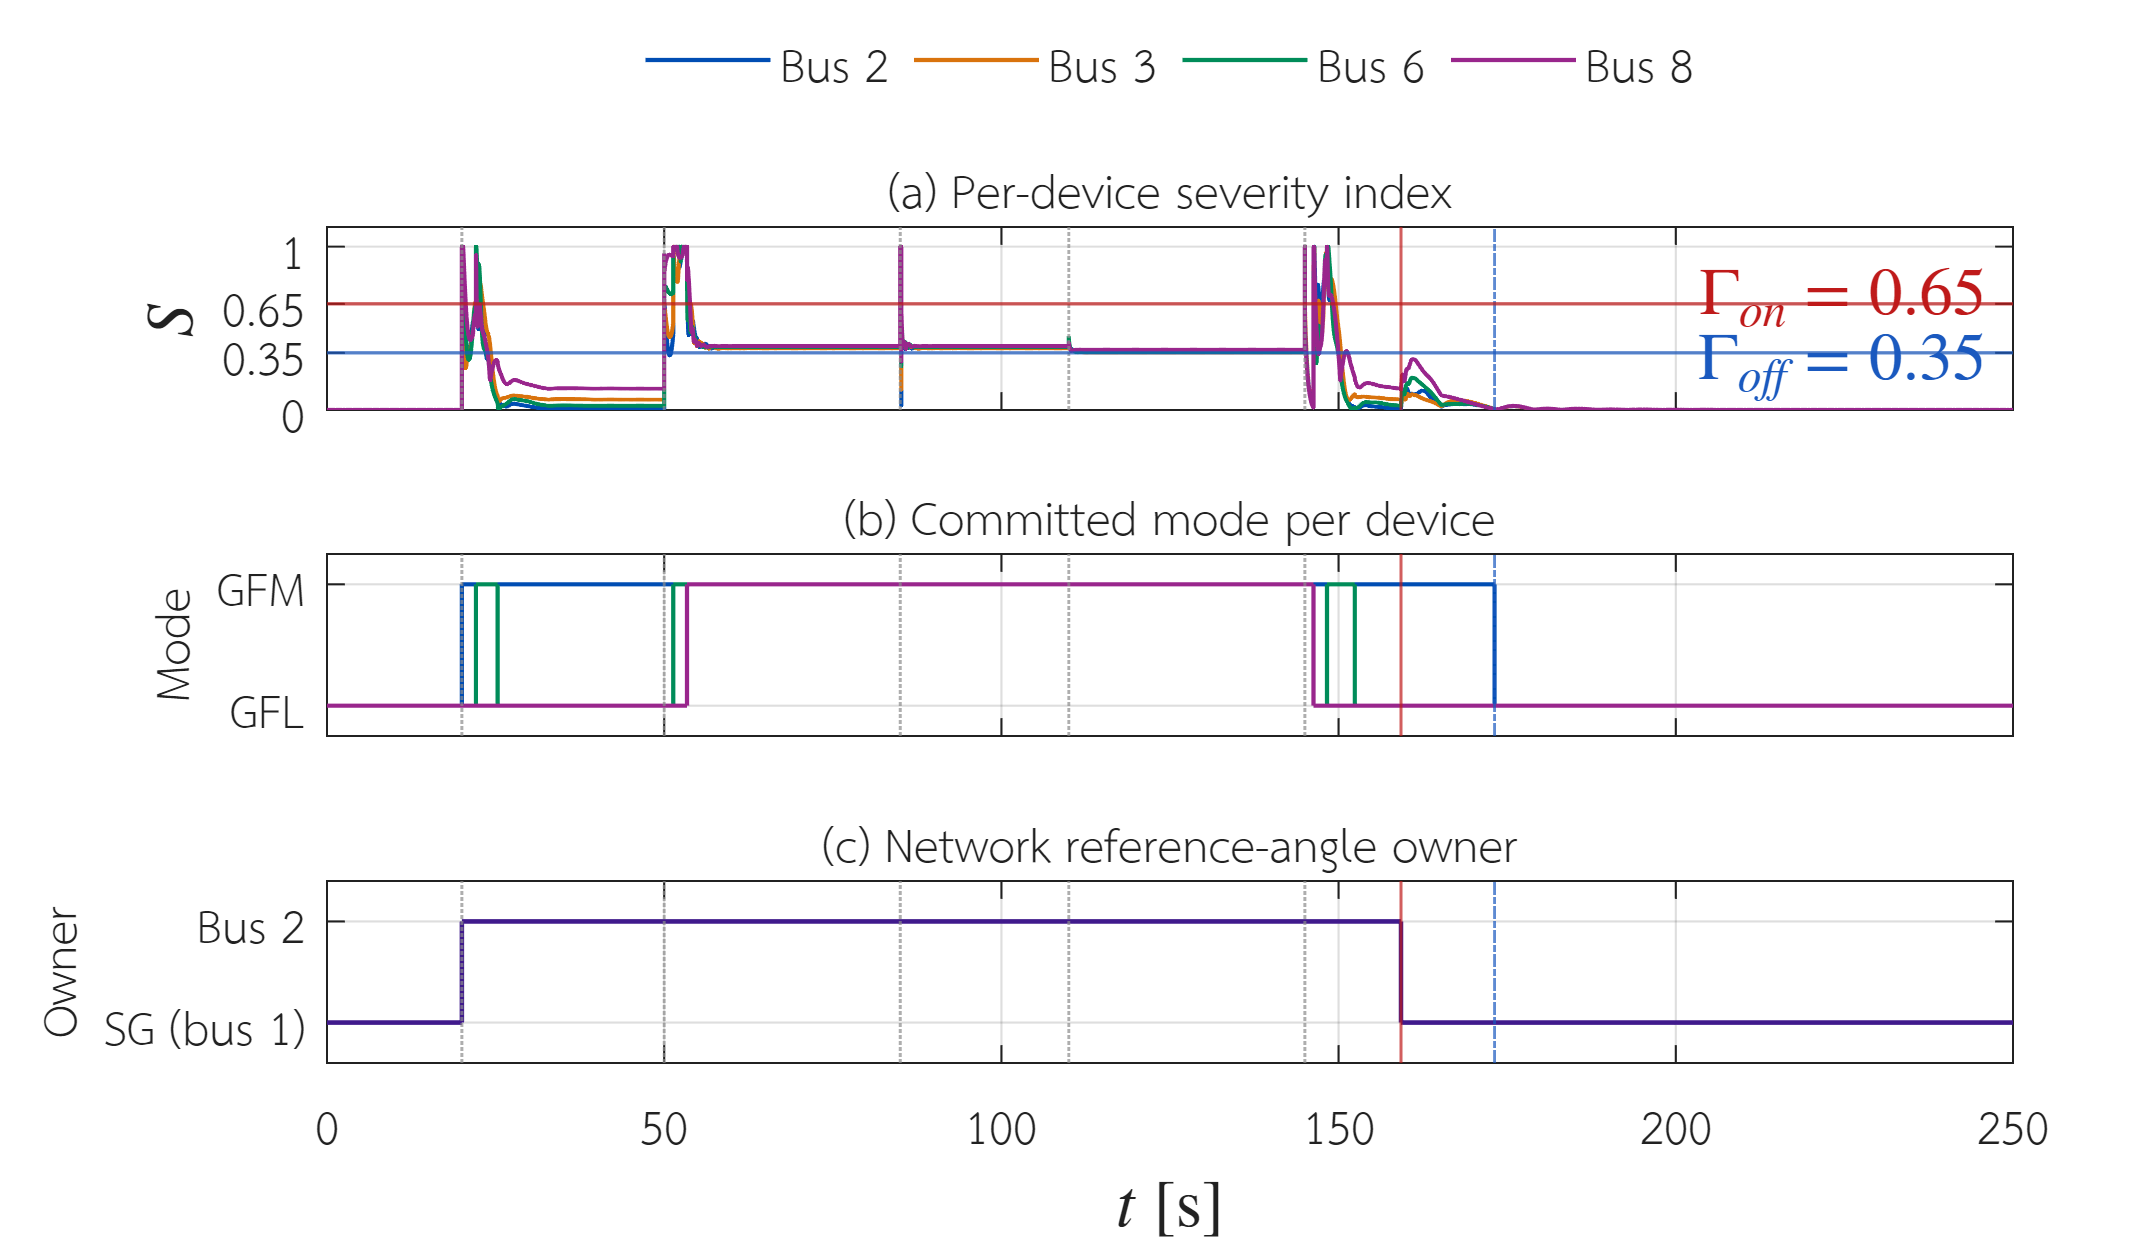
\includegraphics[width=6.20in]{figures/final_report_th/fig_supervisor.png}
\caption{severity, mode และ owner จาก raw adaptive trajectory; สีเป็นเพียงการจัดหมวด}
\end{figure}

\par\vspace{5pt}
% ============================================================================
% 17. Electrical response
\reportsection{ผลตอบสนองไฟฟ้าจาก raw adaptive trajectory}
รูปนี้อ่านจาก trajectory ที่เก็บจริงโดยไม่เติม noise, smoothing, filtering หรือ
การ extrapolate แขนที่หยุดก่อน horizon เส้น event เป็น marker ของเวลาใน schedule
ไม่ใช่การปรับ trajectory ให้เรียบ

\begin{figure}[H]
\centering
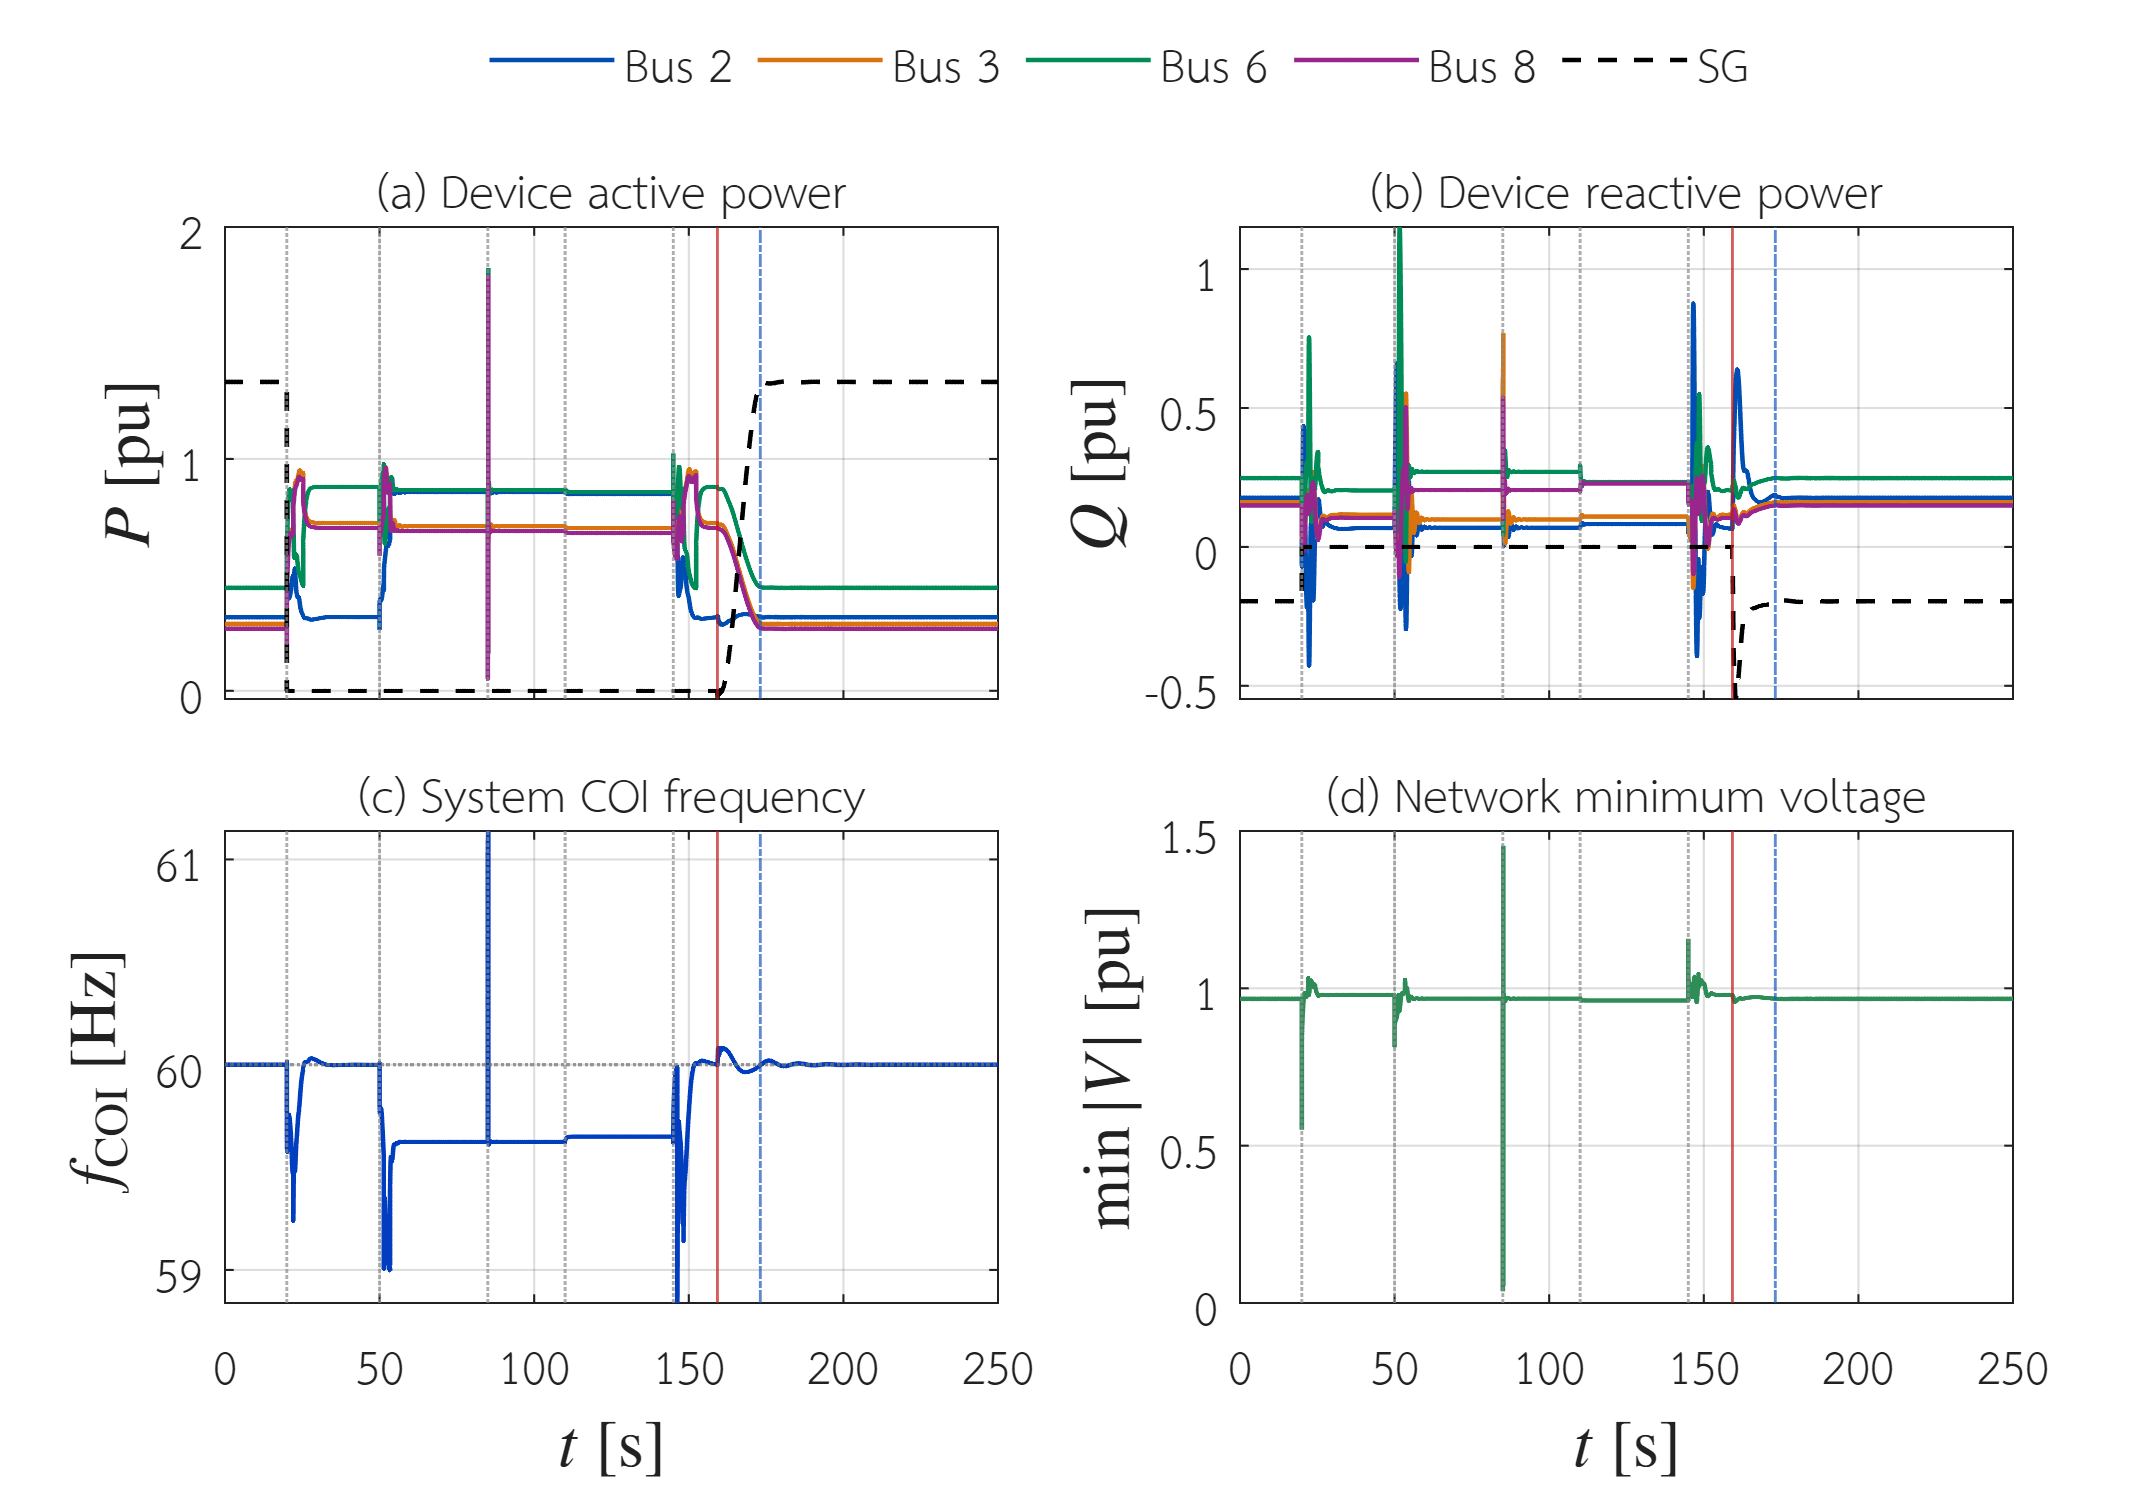
\includegraphics[width=6.20in]{figures/final_report_th/fig_electrical.png}
\caption{กำลัง active/reactive, ความถี่ COI และแรงดันต่ำสุดของ bus ที่ติดตาม}
\end{figure}

\begin{table}[H]
\centering
\caption{ค่าสูงสุด/ต่ำสุดและค่าปลายทางจาก adaptive arm}
\begin{tabularx}{\textwidth}{@{}l r l@{}}
\toprule
ตัวชี้วัด & ค่า & ความหมาย \\
\midrule
$V_{\min}$ ทั้ง trajectory & \NewRunVMin\pu & peak metric \\
$V_{\max}$ ทั้ง trajectory & \NewRunVMax\pu & peak metric \\
$f_{\min}$ ทั้ง trajectory & \NewRunFMin\hz & peak metric \\
$f_{\max}$ ทั้ง trajectory & \NewRunFMax\hz & peak metric \\
$V_{\min},V_{\max}$ ที่ปลายทาง & \NewRunTerminalVMin\pu,\ \NewRunTerminalVMax\pu & settled metric \\
$f$ ที่ปลายทาง & \NewRunTerminalF\hz & settled metric \\
\bottomrule
\end{tabularx}
\end{table}

ช่วง peak สะท้อน disturbance ทั้งหมด ขณะที่ settled metrics อ่านเฉพาะ accepted
sample สุดท้าย จึงไม่ควรนำสองกลุ่มนี้ไปปะปนกัน ค่า residual ของ run คือ
\NewRunResidual\ และไม่มี subdivision เพิ่มใน summary

\par\vspace{5pt}

% ============================================================================
% 18. Six-arm comparison
\reportsection{ตาราง six-arm และการเปรียบเทียบนโยบาย}
แขนทั้งหกอ่านจาก cache ชุดเดียวและผ่าน hash check ก่อนสร้างตาราง จึงแยก
\source{PROJECT\_RESULT} ของแต่ละ policy ออกจากสมมติฐานของตัว solver ได้
ชัดเจน แขนที่หยุดก่อน 250 วินาทีไม่ถูก extrapolate ให้ครบ horizon

\begin{table}[H]
\centering
\caption{ผลการรันหกแขนจาก snapshot เดียว}
\begin{tabularx}{\textwidth}{@{}l r l r r r X@{}}
\toprule
แขน & horizon (s) & สถานะ & reclose (s) & GFM สูงสุด & samples & หมายเหตุ \\
\midrule
\ArmAdaptiveLabel & \ArmAdaptiveHorizon & สำเร็จ & \ArmAdaptiveReclose &
\ArmAdaptiveGfmMax & \ArmAdaptiveSamples & adaptive policy \\
\ArmPinnedgfmOneLabel & \ArmPinnedgfmOneHorizon & สำเร็จ & \ArmPinnedgfmOneReclose &
\ArmPinnedgfmOneGfmMax & \ArmPinnedgfmOneSamples & pin หนึ่งตัว \\
\ArmPinnedgfmTwoLabel & \ArmPinnedgfmTwoHorizon & สำเร็จ & \ArmPinnedgfmTwoReclose &
\ArmPinnedgfmTwoGfmMax & \ArmPinnedgfmTwoSamples & pin สองตัว \\
\ArmPinnedgfmFourLabel & \ArmPinnedgfmFourHorizon & หยุดก่อน horizon & -- &
\ArmPinnedgfmFourGfmMax & \ArmPinnedgfmFourSamples & minimum-step failure \\
\ArmLockedgflLabel & \ArmLockedgflHorizon & หยุดเมื่อ source หาย & -- &
\ArmLockedgflGfmMax & \ArmLockedgflSamples & ไม่มี voltage-forming source \\
\ArmNoadaptationLabel & \ArmNoadaptationHorizon & สำเร็จ & \ArmNoadaptationReclose &
\ArmNoadaptationGfmMax & \ArmNoadaptationSamples & ไม่มี adaptive stepper \\
\bottomrule
\end{tabularx}
\end{table}

\paragraph{Peak กับ settled}
สำหรับ adaptive arm peak voltage range คือ
$[\NewRunVMin,\NewRunVMax]\pu$ และ peak frequency range คือ
$[\NewRunFMin,\NewRunFMax]\hz$ ตลอด trajectory
ค่าปลายทางคือ voltage range
$[\NewRunTerminalVMin,\NewRunTerminalVMax]\pu$ และ
frequency \NewRunTerminalF\hz\ การรายงานสอง envelope แยกกันป้องกัน
การตีความว่า transient peak เป็น operating point สุดท้าย

\begin{figure}[H]
\centering
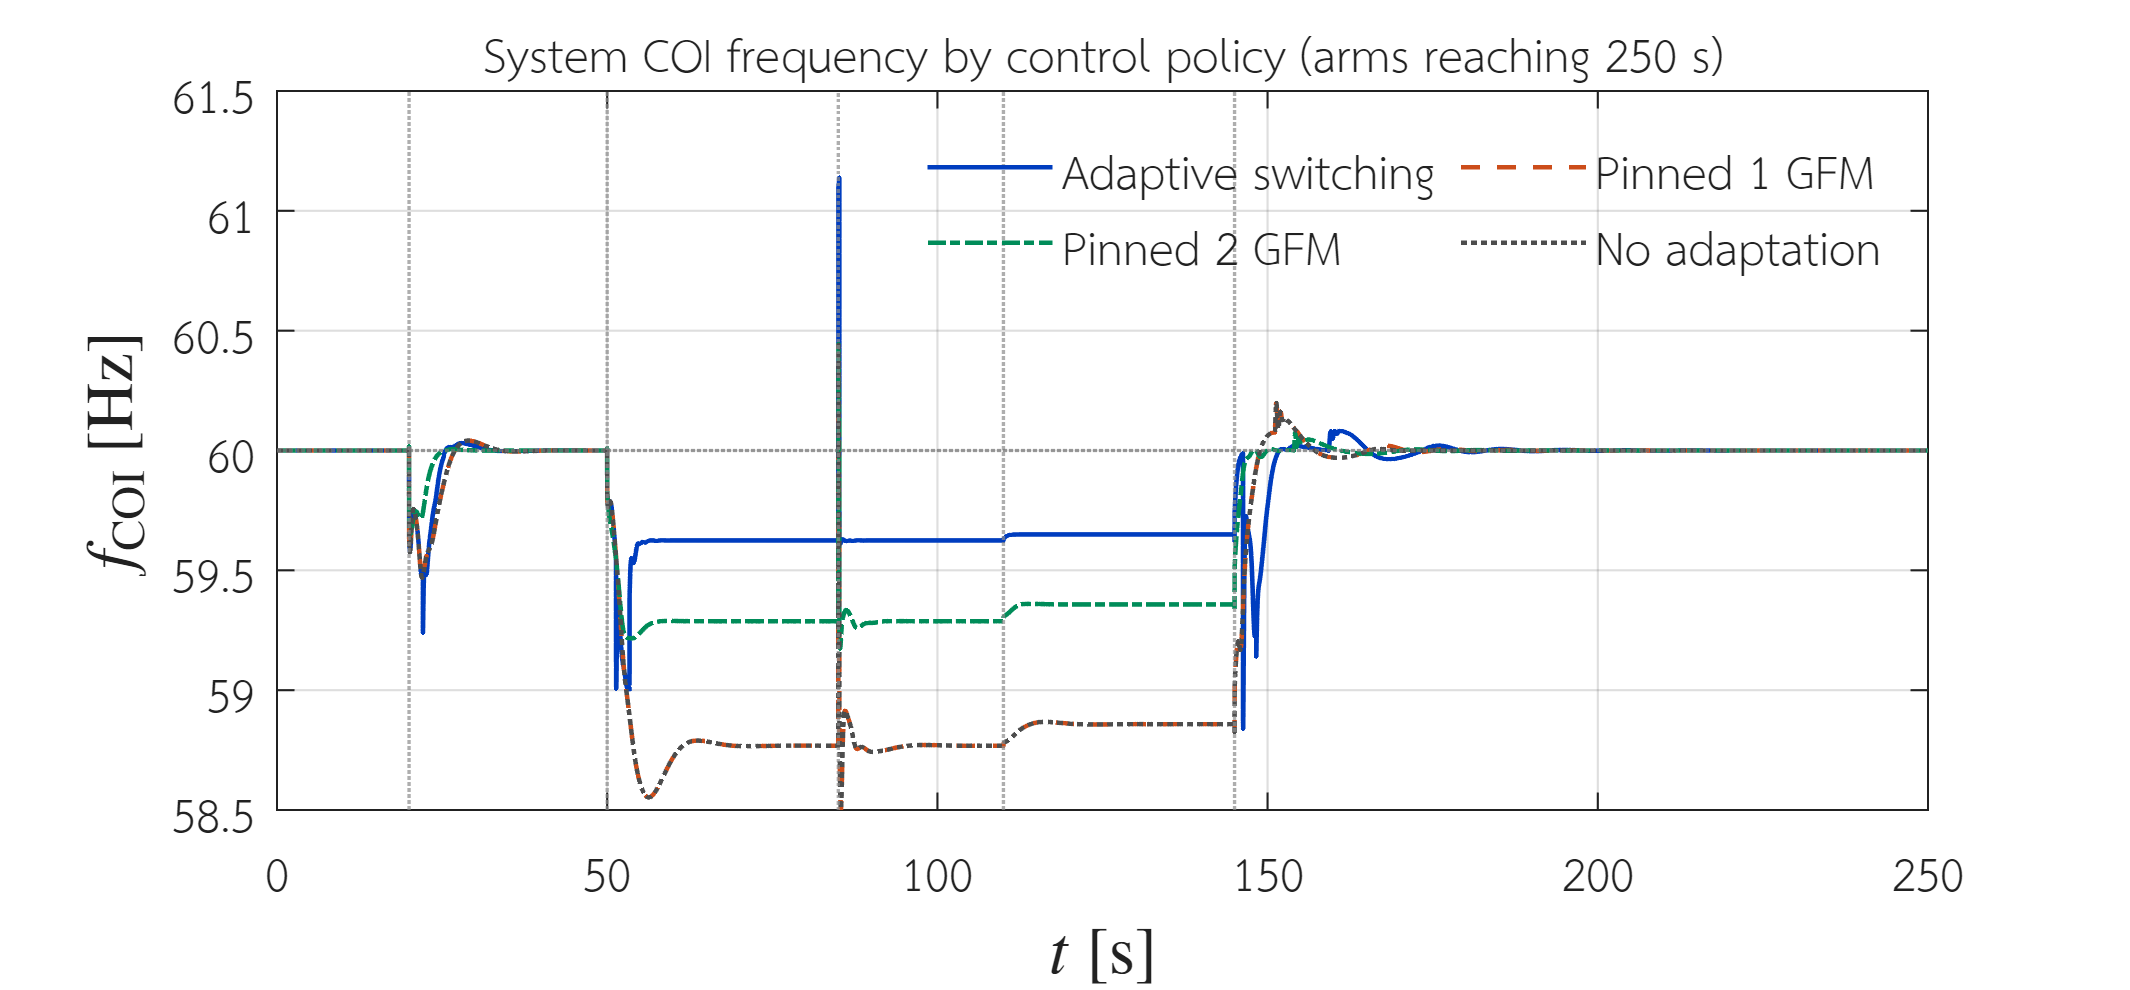
\includegraphics[width=6.20in]{figures/final_report_th/fig_policy.png}
\caption{ความถี่ COI ของแต่ละ policy บนช่วงที่มีข้อมูลจริง; สีแยก policy เท่านั้น}
\end{figure}

ช่วง common window คือ $[0,\CommonWindowSplit)$ วินาที และ
\CommonWindowAllBitIdentical\ หมายถึงทุกแขนที่มีข้อมูลในช่วงนี้ bit-identical
กับ reference; pairwise check แต่ละแขนใช้ \CommonWindowPinnedgfmOneSamples\
ตัวอย่าง ไม่มีการยืดช่วงของแขนที่ล้มเหลว

\par\vspace{5pt}
% ============================================================================
% 19. Limitations, conclusion and references
\reportsection{ข้อจำกัด ความพร้อม ข้อสรุป และเอกสารอ้างอิง}
\paragraph{ข้อจำกัดของข้ออ้าง}
ผลนี้เป็น numerical evidence ของ PF--SSSA--TS และการสลับ mode ใน balanced
RMS model ไม่ใช่การรับรอง EMT, unbalanced protection, hardware controller,
grid-code compliance หรือการใช้งานภาคสนาม ค่าความต่างกับ Padiyar สูงสุดราว
$\sci{4.3}{-2}$ เป็น diagnostic ที่ยังไม่ทราบสาเหตุและไม่ใช่ gate ส่วน PGAz
มี execution artifact แต่ comparison gate ไม่ผ่าน จึงไม่ถูกใช้เป็นหลักฐาน
primary

\paragraph{ความพร้อมของ implementation}
production ใช้สมการและ state order ภายในโครงการ รวมถึง implicit trapezoidal
TS และ Schur solve ด้วย backslash; external programs เป็น oracle เท่านั้น
การเปลี่ยน mode ต้องผ่าน finite-state, KCL, conditioning, continuity และ
authenticated provenance gate การไม่มี voltage-forming source หรือ Newton
right-limit ที่ไม่ผ่านจะหยุดแบบ fail-closed

\paragraph{สิ่งที่ยังไม่อ้าง}
ตัวนับ rejected trial ใน search path ถูกตัดออกจากรายงานเพราะ defect record
ยังเปิดอยู่ จึงไม่ใช้ตัวเลขนั้นสนับสนุน readiness หรือ performance ใด ๆ
นอกจากนี้ผล six-arm เป็น snapshot ที่ commit \texttt{c56ff9f} และรูป/ตาราง
สร้างด้วย generator ที่ตรวจ hash; หาก cache เปลี่ยนต้องสร้างรายงานใหม่ทั้งชุด

\paragraph{ข้อสรุป}
สายงานที่เชื่อม PF, equilibrium, SSSA, TS และ supervisor ด้วย residual กับ
state mapping เดียวกันสามารถตรวจสอบย้อนกลับได้ ผล IEEE-14 แสดงว่า adaptive
arm เดินครบ \NewRunEnd\ วินาที, reclose สำเร็จที่ \NewRunReclose\ วินาที และ
กลับ mode ที่ \NewRunModeReselectionTime\ วินาที ขณะที่ pinned และ locked
arms แสดงขอบเขต failure อย่างซื่อสัตย์ ตาราง six-arm จึงใช้บอก trade-off
ของ policy ไม่ได้ใช้เป็นคำรับรองความมั่นคงเชิงปฏิบัติการ

\paragraph{เอกสารอ้างอิงใน repository}
\begin{enumerate}
\item โครงการ, \textit{Project contracts and numerical integrity},
      \texttt{AGENTS.md}, revision ที่ใช้กับรายงานนี้
\item โครงการ, \textit{IBR reduced-6 EECON49 manifest},
      \texttt{docs/project/IBR\_REDUCED6\_EECON49\_MANIFEST.md}
\item โครงการ, \textit{SSSA validation artifact},
      \texttt{output/validation/artifacts/sssa\_validation.md}
\item โครงการ, \textit{IEEE-14 three-way TS comparison},
      \path{docs/source/figures/case14_ts/case14_ts_compare_three_way.md}
\item โครงการ, \textit{SMIB GFL-RMS10 and GFM-no-PLL diagnostics},
      \texttt{output/diagnostics/smib/}
\item โครงการ, \textit{PF, SSSA, TS and IBR source implementations},
      \texttt{+pfsolver/}, \texttt{+stability/}, \texttt{+ibr/}
\end{enumerate}

\begin{center}
\fcolorbox{navy}{lightblue}{\begin{minipage}{0.91\textwidth}
รายงานฉบับนี้แสดงตัวเลขจาก artifact ที่ตรวจ provenance ได้ แยก
CASE\_DEFINED, PROJECT\_RESULT และ ASSUMED\_DIAGNOSTIC และไม่อ้างค่าที่
ยังอยู่ใน defect state เปิด
\end{minipage}}
\end{center}

\end{document}

